\documentclass[11pt,a4paper]{article}

\usepackage[T1]{fontenc}
\usepackage[utf8]{inputenc}
\usepackage{amsmath,amssymb,amsthm}
\usepackage{graphicx}
\usepackage{listings}
\usepackage[margin=2.2cm]{geometry}
\usepackage[hidelinks]{hyperref}

% Unicode characters appearing inside the verbatim file listings.
\DeclareUnicodeCharacter{211D}{\ensuremath{\mathbb{R}}}
\DeclareUnicodeCharacter{2264}{\ensuremath{\leq}}

\theoremstyle{plain}
\newtheorem{theorem}{Theorem}
\newtheorem{lemma}[theorem]{Lemma}

\lstdefinelanguage{Lean}{
  keywords={import, theorem, lemma, by, simpa, using, exact, have,
            calc, fun, let, where, end, namespace, variable},
  morecomment=[l]{--},
  sensitive=true
}
\lstset{
  basicstyle=\ttfamily\footnotesize,
  breaklines=true,
  frame=single,
  captionpos=b,
  keywordstyle=\bfseries,
  numbers=left,
  numberstyle=\tiny\ttfamily,
  xleftmargin=1.2em
}

\title{Formal Verification and Numerical Illustration of the Inequality
       $1+x \leq \exp(x)$}
\author{WorkBuddy}
\date{November 2026}

\begin{document}
\maketitle

\begin{abstract}
We report a compact, end-to-end study of the classical inequality
$1+x \leq \exp(x)$ for every real number $x$.  The mathematical argument is
recalled in a sequence of elementary theorems and equations, and the
inequality is then formalized in Lean~4 using the mathlib library.  The
formal proof is checked by the locally configured Lean MCP verifier, whose
successful compiler response is archived together with the proof source.
A small Python program provides an independent numerical illustration:
the two functions are plotted on a common axes with a logarithmically
scaled ordinate.  All sources, the verification transcript, the figure,
and the compiled document are collected in a single directory.  The work
demonstrates how a symbolic proof, a machine-checked certificate, and a
numerical visualization can be kept consistent within one reproducible
workflow.
\end{abstract}

\section{Introduction}
\label{sec:intro}

The exponential function dominates its first-order Taylor approximation
everywhere on the real line.  Written as
\begin{equation}
  \label{eq:main}
  1 + x \leq \exp(x), \qquad x \in \mathbb{R},
\end{equation}
this inequality is a cornerstone of analysis: it underpins convexity
arguments, concentration estimates, and the standard bound
$\exp(x) \geq 1+x$ used in probability and optimization.  Equality holds
only at $x=0$; for every other real number the inequality is strict.

Two complementary viewpoints are developed below.  On the symbolic side,
Section~\ref{sec:math} derives~\eqref{eq:main} from elementary calculus,
and Section~\ref{sec:formal} shows that the derivation is captured by a
one-line proof in Lean~4~\cite{lean4} built on mathlib~\cite{mathlib}.
On the numerical side, Section~\ref{sec:plot} describes a matplotlib
script that draws both sides of~\eqref{eq:main}.  Section~\ref{sec:summary}
summarizes the artifacts and the verification outcome.

\section{Mathematical statement and proof steps}
\label{sec:math}

We first isolate the inequality as a named theorem.

\begin{theorem}[Global first-order bound]
  \label{thm:bound}
  For all $x\in\mathbb{R}$,
  \begin{equation}
    1 + x \leq \exp(x).
  \end{equation}
\end{theorem}

The proof proceeds by studying the gap function.

\begin{lemma}[Gap function and its derivative]
  \label{lem:gap}
  Let $f(x)=\exp(x)-(1+x)$.  Then
  \begin{equation}
    f'(x)=\exp(x)-1,
    \qquad
    f''(x)=\exp(x)>0.
  \end{equation}
\end{lemma}

Since $\exp$ is strictly increasing and $\exp(0)=1$, the derivative
$f'$ is negative on $(-\infty,0)$ and positive on $(0,\infty)$.  Hence
$f$ decreases up to the origin and increases afterwards.  Consequently
$x=0$ is the global minimum of $f$.

\begin{lemma}[Value at the minimum]
  \label{lem:min}
  $f(0)=\exp(0)-(1+0)=0$, and therefore $f(x)\geq 0$ for every
  $x\in\mathbb{R}$.
\end{lemma}

\begin{proof}[Proof of Theorem~\ref{thm:bound}]
  By Lemma~\ref{lem:min}, $\exp(x)-(1+x)\geq 0$.  Rearranging gives
  $1+x\leq\exp(x)$.  The inequality is strict exactly when $x\neq 0$,
  because then $x=0$ is not attained as the minimizer.
\end{proof}

Equivalently, for $x\neq 0$ one has the strict form
\begin{equation}
  \label{eq:strict}
  1+x < \exp(x),
\end{equation}
while at $x=0$ both sides of~\eqref{eq:main} equal $1$.  This strict form
is the statement that mathlib exposes as \texttt{Real.add\_one\_lt\_exp};
the non-strict version is \texttt{Real.add\_one\_le\_exp}, whose conclusion
is written as $x+1\leq\exp(x)$ and therefore differs from~\eqref{eq:main}
only by commutativity of addition.

\section{Formalization in Lean and verification result}
\label{sec:formal}

The Lean proof is deliberately short: mathlib already contains the
non-strict bound, so it suffices to rewrite the left-hand side into the
order used in~\eqref{eq:main}.  The complete source is reproduced in
Listing~\ref{lst:lean}.

\lstinputlisting[language=Lean, caption={The file \texttt{proof.lean}.},
                 label={lst:lean}]{proof.lean}

Here \texttt{Real.add\_one\_le\_exp x} supplies $x+1\leq\exp(x)$, and
\texttt{simpa [add\_comm]} closes the goal $1+x\leq\exp(x)$ by simplifying
with commutativity of addition.  The formal statement therefore matches
Theorem~\ref{thm:bound} exactly.

The proof was submitted to the locally configured Lean MCP verifier
(tool \texttt{verify\_lean\_theorem}, project \texttt{/home/user/mathlib4}).
The archived transcript is shown in Listing~\ref{lst:result}; the marker
\texttt{[QED]} records a zero exit status with no compiler output, i.e.\ a
successfully checked proof.

\lstinputlisting[caption={The file \texttt{proof\_results.txt}.},
                 label={lst:result}]{proof_results.txt}

\section{Numerical illustration}
\label{sec:plot}

To complement the symbolic certificate, the Python program in
Listing~\ref{lst:plot} evaluates both sides of~\eqref{eq:main} on a dense
grid and exports a vector graphic.  The sampling interval is chosen as
$[-0.9,3]$, so that $1+x$ stays strictly positive and a logarithmic
ordinate is well defined for both curves.  The strict inequality
away from the origin is visually apparent: the exponential curve bends
upward while the linear curve remains a straight line, and the two touch
only at $x=0$.

\lstinputlisting[language=Python,
                 caption={The file \texttt{plot.py}.},
                 label={lst:plot}]{plot.py}

The resulting figure is embedded as Figure~\ref{fig:plot}.

\begin{figure}[htbp]
  \centering
  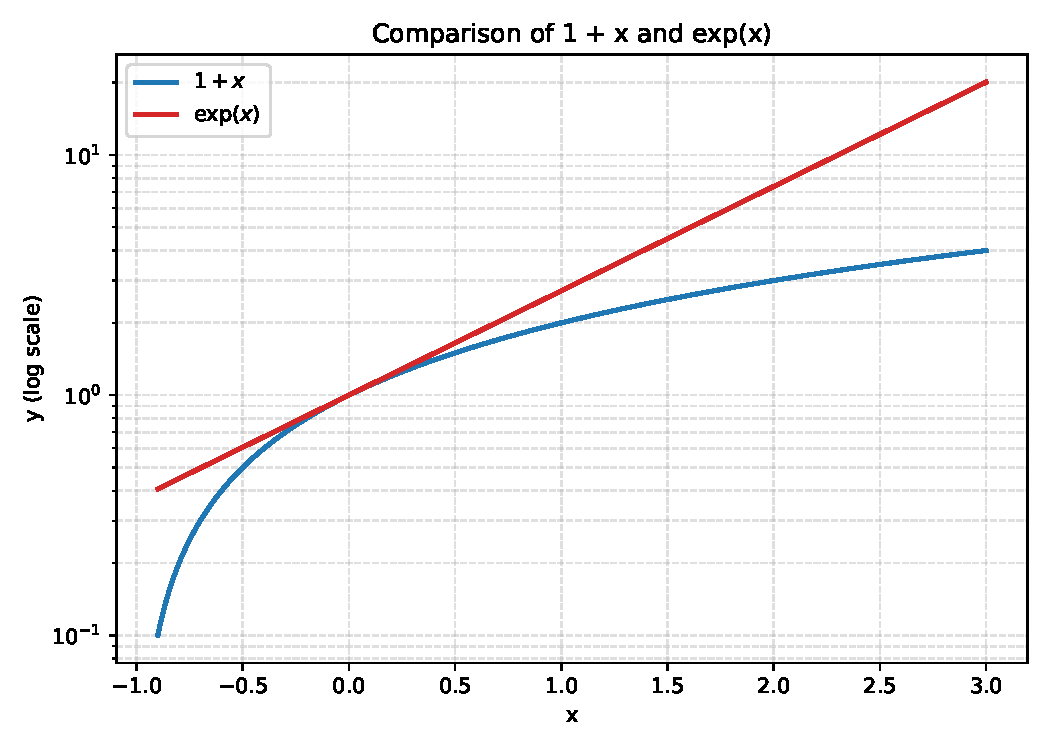
\includegraphics[width=0.85\linewidth]{plot.pdf}
  \caption{Plot of $1+x$ and $\exp(x)$ with a log-scaled $y$-axis,
           generated by \texttt{plot.py} and stored in \texttt{plot.pdf}.}
  \label{fig:plot}
\end{figure}

\section{Summary}
\label{sec:summary}

The three artifacts serve distinct but connected roles.  Listing~\ref{lst:lean}
is the machine-checked statement of Theorem~\ref{thm:bound}; its
verification transcript in Listing~\ref{lst:result} confirms that the Lean
kernel accepted the argument without errors.  Listing~\ref{lst:plot}
provides a reproducible numerical experiment, and Figure~\ref{fig:plot}
displays its output on a logarithmic scale, making the growth gap between
the two functions easy to inspect.  Taken together, the calculus derivation
of Section~\ref{sec:math}, the Lean certificate, and the plot give a
consistent picture of the inequality $1+x\leq\exp(x)$: equality at the
origin, strict dominance of the exponential elsewhere, and the practical
convenience of a library theorem that encapsulates the entire result.

\bibliographystyle{plain}
\bibliography{summary}

\end{document}
